\section{Beading schemes}\label{sec_generalization}
A critical component in toolpath generation is how to distribute the beads over the feature radius.
While the framework presented in the previous section takes evenly distributed beads as an example, it allows to apply different beading schemes to configure the bead distribution to cater for specific requirements from the application, 3D printer or material.



\begin{definition}\label{beading_scheme_definition}
The beading scheme is configured by the following set of functions and constants:
\begin{align*}
\{
&q(d),
B(n, r),
t(n),
t_0(n),
\\
&\alpha_\text{max}, 
t_\text{beading}, 
d_\text{max}^\text{transition}, 
d_\text{max}^\text{unmarked}, 
d_\text{max}^\text{intersection},
d^\text{discretization}
 \}
\end{align*}
where, as introduced in previous section,
$q(d)$ the quantization operator,
$B(n,r)$ is the beading function consisting of $\left( W(n,r), L(n,r) \right)$,
$t(n)$ the transition length,
$t_0(n)$ the transition anchor position,
$\alpha_{\text{max}}$ is the limit bisector angle,
$t_\text{beading}$ is the beading conflict transition length,
$d_\text{max}^\text{unmarked}$ is the filter distance for unmarked regions,
$d_\text{max}^\text{transition}$ is the filter distance for transition anchors,
$d_\text{max}^\text{intersection}$ is the reduction ratio at 3-way intersections
and
$d^\text{discretization}$ is the discretization length in vertex-vertex VD edges and vertex-line VD edges.
%$W(n, r)$ and $L(n, r)$ give the sequence of bead widths $\left\{ w_i \right\}$ and radial locations $\left\{ l_i \right\}$, respectively.
\end{definition}



The following restrictions hold:
\begin{enumerate}
	\begin{minipage}{\columnwidth}
	\setlength\intextsep{0pt}
	\begin{wrapfigure}[4]{o}{.4\columnwidth} %\centering
	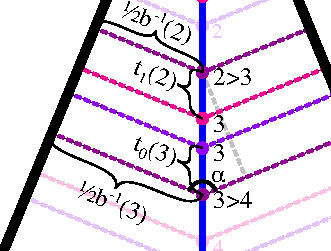
\includegraphics[width=.3\columnwidth,frame]{sources-method-transition-length-limit.pdf}
	%\caption{
	%%Transition ends (magenta and pink) shouldn't cross each other.
	%Placement of transition ends (magenta and pink) with respect to the anchor positions of the transitions (purple) on a ST edge (blue) with bisector angle $\alpha \approx \SI{135}{\degree}$.
	%The distance between the anchor position and the upper end ($t_1$) and the distance between the anchor position and the lower end of the transition ($t_0$) should add up to less than the total distance between the anchor positions, which is limited by $\alpha_\text{max}$.
	%}
	\label{transition_placement}
	\end{wrapfigure}
	\item Transitions shouldn't overlap each other: \\ $t_1(n) + t_0(n+1) < \frac{ q^{-1}(n + 1) - q^{-1}(n) }{ \cos \nicefrac12 \alpha_\text{max}}$ \\ for each $n \in \mathbb{N}$ \\ (see \cref{transition_placement})
\end{minipage}
\item An odd beading should produce an odd single toolpath exactly in the center: $B(n, r)_{\lfloor n/2 \rfloor} = r$ in case $n$ is odd
\item For the smoothness and continuity of toolpaths we require that $W_n$ is monotonic and continuous at each bead index $n$ for constant bead count $c$: $0 \leq \frac{\partial W(c, r)_n}{\partial r} \leq 1$
\end{enumerate}









% \subsection{Beading schemes}
We introduce several beading schemes which determine the bead count and their widths in various ways.
We can emulate a variety of toolpath generation methods from related literature by defining new beading schemes.
We also introduce new beading schemes which produce toolpaths with less extreme widths compared to techniques from existing literature.

A beading scheme is defined as a set of some particular variables and functions (\cref{beading_scheme_definition}).
Our beading schemes are based on a preferred width $w^* = \SI{0.4}{\milli\meter}$, which is equal to the diameter of the printing nozzle.
Most of the beading schemes we introduce share a common ground:
\begin{align*}
L(n,r)_i = 
\begin{cases}
-\frac12 W(n,r)_i + \sum_{j=0}^i W(n,r)_j & \text{ if } i < \frac12 (n -1) \\
r & \text{ if } i =  \frac12 (n -1) \\
%d - W(n,r)_{n-1-i} & \text{ otherwise }\\
\end{cases}
\\
\begin{array}{rlrl}
t_\text{beading} &= w^* 
&
d_\text{max}^\text{transition} &= \SI{1}{\milli\meter}
\\
t(n) &= w^*
&
d_\text{max}^\text{unmarked} &= w^*
\\
t_0(n) &=  t(n) \left( q^{-1}(n) / w^*  - n \right)
&
d^\text{discretization} &= \SI{0.2}{\milli\meter}
\\
\alpha_\text{max} &= \SI{135}{\degree} 
&
d_\text{max}^\text{intersection} &= \SI{75}{\percent}
\end{array}
%\end{align*}
%\begin{align*}
\end{align*}

The toolpath locations $L$ ensure 
that the beads don't overlap,
that beads are extruded from the center of where they end up
and that the symmetry restrictions are met.
The transition anchor position $t_0$ ensures that the transitions never overlap with the locations $v$ where $R(v) = \nicefrac12 n w^*$ for $n \in \mathbb{N}$.
The transition length $t$ ensures that the center beads don't overlap with the innermost transitioning beads, while keeping the amount of underfill low and keeping the toolpath smooth.
The limit bisector angle $\alpha_\text{max}$ ensures that we don't employ transitioning in shallow wedge regions, which would result in a lot of short odd single bead polylines, which would break up the semi-continuous nature of polygonal extrusion paths.




\begin{table}%\centering
\caption{
\revise{Made figure into table}{
Beading schemes.
}
} % revise
\label{beading_schemes}
%
\setlength{\figwidth}{.45\linewidth}
\captionsetup[subtable]{justification=justified,singlelinecheck=false}
%
%
%
\begin{tabular}{|l|l|}
\hline
%
%
\begin{subtable}[b]{\figwidth}
\smallskip
\caption{Uniform scheme}\label{formula_uniform}
$\begin{aligned}
\alpha_\text{max} &= \SI{180}{\degree} \\
q^-(d) &= 2 \left\lfloor \frac{d}{ 2w^*} + \frac12 \right\rfloor \\
W(n,r)_i &= w^* \text{ for all } i 
%\\
%L(n,r)_i &= w^* \left(i + \frac12 \right) \text{ for all } i < \frac12 n
\end{aligned}$
\end{subtable}
%
%
&
%
%
\begin{subtable}[b]{\figwidth}
\smallskip
\caption{Outer bead}\label{formula_outer_bead}
$\begin{aligned}
q(d) &=
\begin{cases}
1 & \text{ if } d < w^* \\
2 & \text{ otherwise } \\
\end{cases}
 \\
W(n,r)_i &= 
\begin{cases}
2r & \text{ if } n = 1 \\
w^* & \text{ otherwise } \\
\end{cases}
%\\
%L(n,r)_i &= 
%\begin{cases}
%2r / 2 & \text{ if } n = 1 \\
%w^* / 2 & \text{ otherwise } \\
%\end{cases}
\end{aligned}$
\end{subtable}
%
%
 \\ \hline
%
%
\begin{subtable}[b]{\figwidth}
\smallskip
\caption{Constant bead count}\label{formula_constant_bead_count}
$\begin{aligned}
\alpha_\text{max} &= \SI{0}{\degree} \\
q(d) &= C \\
W(n,r)_i &= 2 r / n \text{ for all } i 
%\\
%L(n,r)_i &= 2r / n \left(i + \frac12 \right) \text{ for all } i < \frac12 n
\end{aligned}$
\end{subtable}
%
%
&
%
%
\begin{subtable}[b]{\figwidth}
\smallskip
\caption{Evenly distributed}\label{formula_evenly_distributed}
$\begin{aligned}
q(d) &= \left\lfloor \frac{d}{ w^*} + \frac12 \right\rfloor \\
W(n,r)_i &= 2 r / n \text{ for all } i 
%\\
%L(n,r)_i &= 2r / n (i + \frac12) \text{ for all } i < \frac12 n
\end{aligned}$
\end{subtable}
%
%
 \\ \hline
%
%
\multicolumn{2}{|l|}{
\begin{subtable}[b]{\linewidth}
\smallskip
\caption{Centered}\label{formula_centered}
$\begin{aligned}
t(n) &= \frac12 w^* \\
%q^-(d) &= 2 \left\lfloor \frac{d}{ 2w^*} + \frac12 \right\rfloor \\
q(d) &= q^-(d) +
\begin{cases}
-1 & \text{ if } q^-(d) w^* - d > w^* - r_\text{max} \\
1  & \text{ if }  q^-(d) w^* - d < w^* - r_\text{min} \\
0 & \text{ otherwise}
\end{cases}
\\
W(n,r)_i &= 
\begin{cases}
2 r - (n-1) w^* &\text{ if } i = \frac12 (n-1) \\
w^* &\text{ otherwise }
\end{cases}
%\\
%L(n,r)_i &= 
%\begin{cases}
%2r / 2 & \text{ if } i = \frac12 (n-1) \\
%w^* \left(i + \frac12 \right) & \text{ otherwise }
%\end{cases}
\end{aligned}$
\end{subtable}
}
%
%
 \\ \hline
%
%
\multicolumn{2}{|l|}{
\begin{subtable}[b]{\linewidth}
\smallskip
\caption{Inward distributed}\label{formula_inward_distributed}
$\begin{aligned}
q(d) &= \left\lfloor \frac{d}{ w^*} + \frac12 \right\rfloor \\
E(n,r) &= 2r - n w^* \\
W(n,r)_i &= w^* + E(n,r) \frac{\omega(n,r)_i}{\sum_{j=0}^{n-1} \omega(n,r)_j} \text{ for all } i \\
%L(n,r)_i &= 2r / n (i + \frac12) \text{ for all } i < \frac12 n
\omega(n,r)_i &= \max(0, 1 - N^{-2} (i - (n-1)/2)^2 )
\end{aligned}$
\end{subtable}
}
 \\ \hline
%
%
\end{tabular}
\end{table}


\paragraph{Uniform beading scheme}
We can define a beading scheme which emulates the uniform width offsetting technique by disabling the marking of edges, so that we never employ transitioning.
See \cref{formula_uniform}.


\paragraph{Outer bead}
We can emulate the method from \citeauthor{Moesen2011} by carefully choosing how the beading scheme functions deal with the outermost bead.
Also we turn off the reduction of toolpaths near 3-way intersections $d_\text{max}^\text{intersection} = \SI{0}{\percent}$, so that the polygonal toolpaths emulate the remaining area to be filled by another path planning technique similar to their technique.
We don't need transitioning, so we also set $t(n) = 0 $.
See \cref{formula_outer_bead}.



\paragraph{Constant bead count}
We can emulate the method from \citeauthor{Ding2016a} by dividing the feature radius over the widths of a constant number of beads.
Additionally in order to emulate their definition of ``branches'' we mark all ST edges we unmark the outer edges connected to the outline shape in a separate algorithm.
Note that this deviation from the proposed framework violates the robustness against small perturbations in the outline polygon, since this marking depends on the topology of the graph of the ST.
See \cref{formula_constant_bead_count}.




\paragraph{Centered}
We can emulate the method from \citeauthor{Jin2017JMS} by transcribing how they deviate from the uniform width toolpaths.
We therefore base the beading scheme on the bead count $q^-(d)$ defined by the uniform beading scheme.
\citeauthor{Jin2017JMS} replace two beads from the uniform toolpaths by a single one when the radius between the center and either of those beads falls short of $r_\text{min} = 0.8 w^*$.
Conversely, they place an extra bead when the radius between the center and either of the innermost beads exceeds $r_\text{max} = 1.25 w^*$~\cite{Jin2017JMS}.
We emulate the rounded polygonal path rerouting they define by supplying a transition length which results in a discretized version of the rounded polygon segment.
See \cref{formula_centered}.






\paragraph{Evenly distributed}
By taking the advantages of the above two schemes we can define a beading scheme which constitutes a novel toolpathing technique.
We can evenly divide the local feature diameter over the widths of all beads, but choose a local bead count better matching the local feature size.
We determine the local bead count by dividing the diameter by the preferred bead width and rounding to the nearest integer.
This reduces the demands on the system and deviation from mechanical properties caused by beads with extreme deviations from the preferred width.
See \cref{formula_evenly_distributed}.






\paragraph{Inward distributed scheme}
The evenly distributed scheme can be conceptualized as calculating the total discrepancy $E$ between the actual feature diameter $d$ and the total preferred width $n w^*$, dividing the total discrepancy by the number of beads and setting the width of each bead to 
$w^* + E / n$.
However, depending on the application we might want a different distribution of widths.
We therefore supply a beading scheme which supports an arbitrary distribution of the discrepancy.
The distribution is determined by some weighing function $\omega(n,r)$, which defines the portion of the discrepancy to distribute to each bead.
%\paragraph{Inward distributed}
See \cref{formula_inward_distributed}.
For example, we can choose an $\omega$ which distributes the discrepancy over the innermost $N$ beads, and distribute most of it to the inner beads.
See \cref{distributed_comparison}.
That way we limit the region of impact of the distributed scheme to a central region and have the preferred bead width $w^*$ in regions farther away.
This limits the impact of transitioning regions so that transitions keep the toolpaths smooth farther away from the central regions. % and it forces most of the beads to have exactly the preferred width.
%Moreover, the bead widths equal the preferred bead width for large regions meaning that mechanical properties derived for prints using the uniform scheme will still hold approximately.






\begin{figure}
\centering
\setlength{\figwidth}{.4\columnwidth}
\setlength{\figheight}{.25\columnwidth}
\begin{subfigure}[t]{\figwidth}\centering
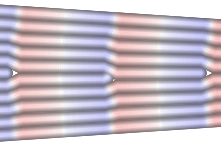
\includegraphics[height=\figheight,frame]{sources-validation-wedge-Distributed-pretty-evenly.png}
\caption{Evenly distributed}
\end{subfigure}
\begin{subfigure}[t]{\figwidth}\centering
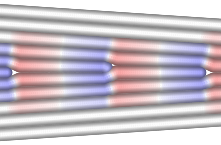
\includegraphics[height=\figheight,frame]{sources-validation-wedge-Distributed-pretty-inward.png}
\caption{Inward distributed}
\end{subfigure}
\begin{subfigure}[t]{.1\columnwidth}\centering
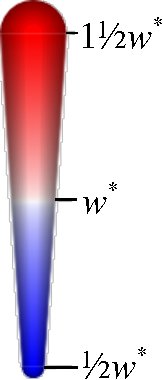
\includegraphics[height=\figheight]{sources-validation-widths-legend-small.pdf}
\end{subfigure}
\caption{
Closeup of toolpaths generated with the distributed beading schemes for a large wedge shape.
Colors represent bead widths.
}
\label{distributed_comparison}
\end{figure}








\paragraph{Widening \revise{}{meta-scheme}}
Complementary to any of these schemes we can enforce a minimum feature size at no extra cost in our framework.
Regions where the model is narrower than some $r_\text{min}$ can be printed with a bead width $w_\text{min}$ larger than the model thickness.
In order to get results such as in \cref{widening} we can override
\begin{align*}
q'(d) &= 
\begin{cases}
0 & \text{ if } 0 \leq d < 2 r_\text{min} \\
1 & \text{ if }  2 r_\text{min} \leq d < w^*  \\
q(d) & \text{ otherwise}
\end{cases}
\\
W'(n,r)_0 &=
\begin{cases}
\max \left( w_\text{min}  ,  2 r \right) & \text{ if } 2 r < w^* \\
W(n,r)_0 & \text{ otherwise}
\end{cases}
\end{align*}



\revise{}{
\paragraph{Shell meta-scheme}
The industry standard of FDM is to generate only a limited contour-parallel perimeters and to fill the remainder using a direction-parallel strategy.
We therefore provide a meta-scheme to generate adaptive bead width toolpaths only in narrow regions and generate the limited number of perimeters $M$ using the preferred width in regions which are wide enough.
We also take care not to leave gaps which are too small to be filled using the direction-parallel strategy:

\begin{align*}
q'(d) &= \min(M, q(d))
\\
W'(n,r)_i &= 
\begin{cases}
W(n, M w^*)_i & \text{ if } 2 r > q^{-1}(M) \\
W(n,r)_i & \text{ otherwise}
\end{cases}
\end{align*}

These meta-schemes introduce non-linearities in the quantization function.
Because the beading is only evaluated at nodes in the skeleton, we need to make sure that there are nodes at the locations along the skeleton where the non-linearities happen.
We therefore insert extra nodes along with their ribs at locations $v$ with a radial distance $R(v) = r_\text{min}$ for widening and at $R(v) \in \left\{ M w^*, q^{-1}(M), q^{-1}(M) + \nicefrac12 w^* \right\} $ for the transition from narrow shell to unconstrained shell.
Combining all meta-schemes functionality we can generate results such as depicted in \cref{widening_shell}.

\begin{figure}
\centering
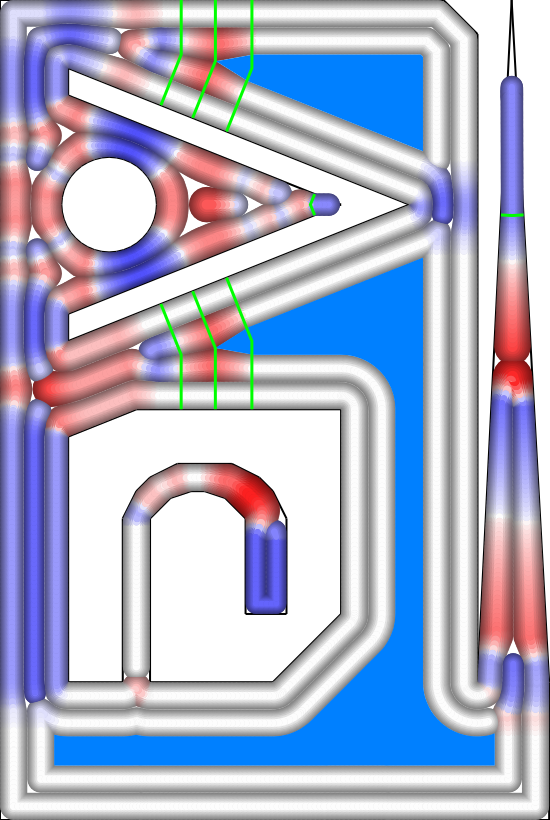
\includegraphics[rotate=90,width=.6\columnwidth]{sources-validation-gMat_example_all_combined.png}
\caption{
Toolpath generated with the inward distributed strategy ($N=1.5$) in conjunction with the widening meta-scheme ($W_\text{min}=0.5, 2r_\text{min}=0.2$, see top left) and the shell meta-scheme ($M=4$, see middle).
% -p test_geometry/gMAT_example.svg -b 4 -s i -n 1.5 -a --mins 0.2 --minw .5
Widening and shell require extra edges (green) at key locations in the skeleton.
The azure area is to be filled using some direction-parallel toolpath generation algorithm.
}
\label{widening_shell}
\end{figure}
}
















